\documentclass[11pt]{beamer}
\author{Philipp Arras, Florian Nowak}
\title{\LaTeX -Kurs}
\date{11. Oktober 2014}

\usetheme{Berkeley}
%\setbeamercovered{transparent}
\setbeamertemplate{navigation symbols}{}
%\logo{}
%\institute{}
%\subject{}

\usepackage[utf8]{inputenc}
\usepackage[ngerman]{babel}
\usepackage{amsmath,amsfonts,amssymb}
\usepackage{graphicx,booktabs}

\usepackage{pdfpages,wasysym}

\begin{document}

%\begin{frame}
%\titlepage
%\end{frame}

%\begin{frame}
%\tableofcontents
%\end{frame}

\section{Tabellen und Figuren}
\begin{frame}{Was sind Gleitobjekte?}
\begin{itemize}
\item Objekte, die frei im Dokument {\glqq}gleiten{\grqq} können
\item Gleiten vermeidet große Leerräume
\item {\TeX} \emph{versucht} optimale Positionierung
\end{itemize}
\end{frame}

\begin{frame}[fragile]{Gleitumgebungen}
\textbf{Eine Gleitumgebung vesteht aus verschiedenen Teilen}
\begin{itemize}
\item Inhalt (Bild, Tabelle, Text, o. ä.)
\item Bezeichnung mit Nummerierung: {\glqq}Tabelle 1:{\grqq} (\verb~\caption~)
\item Beschriftung: {\glqq}Messergebnisse{\grqq}\\
(Argument von \verb~\caption{...}~)
\item Markierung für Verweise: \verb~\label{fig:messergebnisse}~
\end{itemize}
\end{frame}

\begin{frame}[fragile]{Gleitumgebungen}
\textbf{Eine Gleitumgebung vesteht aus verschiedenen Teilen}
\begin{itemize}
\item Inhalt (Bild, Tabelle, Text, o. ä.)
\item Bezeichnung mit Nummerierung: {\glqq}Tabelle 1:{\grqq} (\verb~\caption~)
\item Beschriftung: {\glqq}Messergebnisse{\grqq}\\
(Argument von \verb~\caption{...}~)
\item Markierung für Verweise: \verb~\label{tab:messergebnisse}~
\item[$\Rightarrow$] Verweis anschließend durch\\
{\glqq}\verb!siehe Tabelle~\ref{tab:messergebnisse}.!{\grqq}
\end{itemize}
\end{frame}

\begin{frame}{Gleitumgebungen}
\textbf{{\LaTeX} verfügt über verschiedene Gleitumgebungen}
\begin{itemize}
\item \texttt{table} für Tabellen
\item \texttt{figure} für Abbildungen
\item Eigene Umgebungen können mit dem \texttt{float}-Paket definiert werden 
\end{itemize}
\end{frame}

{
\setbeamercolor{background canvas}{bg=}

\includepdf[pages=7]{06-Gleitumgebungen-I}
}

{
\setbeamercolor{background canvas}{bg=}

\includepdf[pages=15]{06-Gleitumgebungen-I}
}

\begin{frame}[fragile]{Standard-Tabellenumgebung: tabular}
\textbf{Beispiel: Das hier}
\begin{verbatim}
\begin{table}[h]
  \label{tab:1}
  \caption{Erstkontakt}
  \begin{tabular}{lcr}
    links & zentriert & rechts \\
    auch links & wieder zentriert & erneut rechts
  \end{tabular}
\end{table}
\end{verbatim}
\end{frame}

\begin{frame}[fragile]{Standard-Tabellenumgebung: tabular}
\textbf{liefert}
%\begin{verbatim}
\begin{table}[h]
  \label{tab:1}
  \caption{Erstkontakt}
  \begin{tabular}{lcr}
    links & zentriert & rechts \\
    auch links & wieder zentriert & erneut rechts
  \end{tabular}
\end{table}
%\end{verbatim}
\end{frame}

{
\setbeamercolor{background canvas}{bg=}

\includepdf[pages=17-21]{06-Gleitumgebungen-I}
}

\begin{frame}[fragile]{Standard-Abbildungsumgebung: figure}
\textbf{Beispiel: Dies hingegen}
\begin{verbatim}
\begin{figure}[h]
  \label{fig:1}
  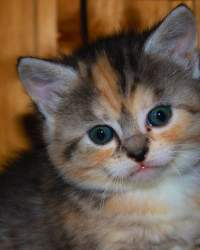
\includegraphics[scale=.5]{250}
  \caption{pussy close-up}
\end{figure}
\end{verbatim}
\end{frame}

\begin{frame}[fragile]{Standard-Abbildungsumgebung: figure}
\textbf{liefert}
%\begin{verbatim}
\begin{figure}[h]
  \label{fig:1}
  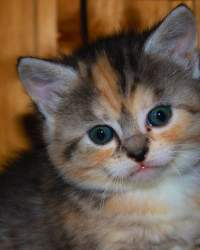
\includegraphics[scale=.5]{250}
  \caption{pussy close-up}
\end{figure}
%\end{verbatim}
\end{frame}

\begin{frame}[fragile]{Spaß mit graphicx}
\begin{itemize}
\item Das Paket \texttt{graphicx} bietet neben \texttt{scale} weitere optionale Parameter für \verb~\includegraphics[...]{...}~
\end{itemize}
\end{frame}

\begin{frame}[fragile]{Spaß mit graphicx}
\begin{itemize}
\item Das Paket \texttt{graphicx} bietet neben \texttt{scale} weitere optionale Parameter für \verb~\includegraphics[...]{...}~
\item[$\Rightarrow$] Einfach und schnell etwa auf\\
 \url{en.wikibooks.org/wiki/LaTeX/Importing_Graphics} nachschlagbar \smiley
\end{itemize}
\end{frame}

\begin{frame}{Übungen}
\begin{enumerate}
\item Erstellt eine kleine (schöne) Tabelle mit Inhalt eurer Wahl; verwendet dabei \emph{umbedingt} das Paket \texttt{booktabs}! Fasst eure Tabelle in eine \texttt{table}-Umgebung ein und gebt ihr eine Unterschrift. Schreibt einen kurzen Satz (darunter) mit Verweis auf die Tabelle.
\item Ladet euch ein (lustiges) Bild eurer Wahl runter (etwa von \url{http://placekitten.com/}) und fügt es innerhalb einer \texttt{figure}-Umgebung ein. (Unterschrift \emph{nicht} vergessen!) Reskaliert und rotiert das Bild und probiert verschiedene Parameter für eure \texttt{figure} aus; fügt \emph{sowohl} vor \emph{als auch} nach eurer Umgebung (mehrere) \texttt{blindtext} ein um das Verhalten dieser Modifikationen besser zu beobachten!
\end{enumerate}
\end{frame}


\end{document}